\documentclass[conference]{IEEEtran}

\usepackage[T1]{fontenc}
\usepackage[utf8]{inputenc}
\usepackage{amsmath,amssymb}
\usepackage{booktabs}
\usepackage{array}
\usepackage{graphicx}
\usepackage{xcolor}
\usepackage{url}
\usepackage[hidelinks]{hyperref}
\usepackage{enumitem}
\usepackage{tabularx}

\setlist[itemize]{leftmargin=*, itemsep=2pt, topsep=2pt}
\setlist[enumerate]{leftmargin=*, itemsep=2pt, topsep=2pt}
\newcolumntype{Y}{>{\raggedright\arraybackslash}X}

\title{Deep Learning-Based Road Detection, Condition Assessment, and RAG-Assisted Decision Support in Rural Sindh, Pakistan}

\author{\IEEEauthorblockN{Hammadullah Muazzam}
\IEEEauthorblockA{Final Year Project Technical Report\\
Roadlytics: Road Intelligence Studio\\
April 2026}}

\begin{document}
\maketitle

\begin{abstract}
This report documents the complete technical evolution of Roadlytics, an end-to-end system for automated road infrastructure monitoring from Sentinel-2 Level-2 multispectral satellite imagery over rural Sindh, Pakistan. The core machine-learning pipeline addresses two complementary objectives: binary semantic segmentation for road network extraction and pixel-level road-condition classification into Good, Unpaved, and Damaged classes. Across six sequential segmentation experiments, the model evolved from a U-Net/ResNet-34 baseline with 31.4\% test IoU to an optimized configuration using morphological label dilation that achieved 66.2\% test IoU, satisfying the NFR-11 target range of 65--75\%. A parallel DeepLabV3+ investigation with an SE-ResNeXt-101 encoder reached 63.1\% test IoU after extended training with Automatic Mixed Precision. For road-condition assessment, K-Means pseudo-labelling over spectral features provides scalable supervision for an EfficientNet-B2 classifier, which achieves 83\% held-out test accuracy and a macro F1-score of 0.83.

The report has been expanded to include the deployed Roadlytics web platform and its Retrieval-Augmented Generation (RAG) assistant. The application productizes the research pipeline into a FastAPI backend, Next.js frontend, Dockerized deployment, Azure VM runtime, Azure Blob storage integration, map-based raster overlay analysis, report generation, and a grounded assistant layer. The RAG assistant retrieves job metadata, event timelines, artifact manifests, analytics snapshots, generated report text, static method notes, and guardrail documentation through a ChromaDB-backed retrieval service with deterministic local hash embeddings. Gemini generation is used when a Google AI Studio API key is configured; otherwise, the system falls back to extractive evidence-based responses. The assistant supports project-wide summaries, job-scoped explanation, map-layer interpretation, report drafting, failure diagnosis, and decision-support guardrails while explicitly avoiding unsupported claims about field truth, road safety, legal compliance, or repair cost.
\end{abstract}

\begin{IEEEkeywords}
Road segmentation, Sentinel-2, semantic segmentation, U-Net, DeepLabV3+, EfficientNet, K-Means, GeoTIFF, FastAPI, Next.js, Docker, Azure, ChromaDB, Retrieval-Augmented Generation, Gemini.
\end{IEEEkeywords}

\section{Introduction}
Road infrastructure in developing regions faces persistent monitoring challenges, including limited ground-survey capacity, infrequent inspections, and sparse condition records. In rural Sindh, unpaved and deteriorating roads can affect access to markets, schools, healthcare facilities, and emergency response. Conventional survey methods are costly and difficult to repeat at regional scale, creating a strong case for remote-sensing-assisted road assessment.

Roadlytics uses freely available Sentinel-2 imagery and open-source geospatial and machine-learning tooling to create a scalable monitoring workflow. The system began as a model experimentation pipeline and was later productized into a web application. The core analytical workflow contains two model stages. First, a segmentation stage extracts road pixels from a four-band Sentinel-2 GeoTIFF containing B2, B3, B4, and B8 bands. Second, a condition-classification stage assigns road pixels to Good, Unpaved, or Damaged classes. The final web system allows a user to upload a Sentinel-2 GeoTIFF, select segmentation and classification methods, run the pipeline as a background job, inspect the generated raster layers on an OpenStreetMap basemap, and download reports and artifacts.

The primary segmentation success criterion is NFR-11: a test-set IoU in the 65--75\% range. This report documents the experiments that led to that result, the condition-classification strategy, the deployment architecture, and the RAG assistant introduced to make Roadlytics results more interpretable to non-specialist users.

\section{Dataset and Preprocessing}
\subsection{Imagery and Study Area}
Input imagery consists of four-band Sentinel-2 Level-2 composites at 10 m ground sampling distance. The selected bands are Blue (B2), Green (B3), Red (B4), and Near Infrared (B8). The study area covers rural road corridors in Sindh, Pakistan. Binary road masks were prepared from high-resolution reference data and co-registered to the Sentinel-2 grid.

\subsection{Tile Extraction}
A sliding-window procedure extracts square tiles using configurable \texttt{TILE\_SIZE} and \texttt{STRIDE} parameters. Tiles are retained only when they meet a minimum road ratio of \texttt{MIN\_ROAD\_RATIO=0.005}, equivalent to 0.5\%. This prevents the training set from being dominated by nearly empty background tiles. The resulting catalogue is split into 70\% training, 15\% validation, and 15\% testing subsets using a fixed random seed of 42 for reproducibility.

\subsection{Class Imbalance}
Road pixels constitute fewer than 2\% of all pixels, creating a severe foreground-background imbalance. Three complementary strategies were used: stratified tile filtering, a combined Focal-Dice loss, and a reduced prediction threshold in the range $\tau=0.3$--$0.5$ to improve recall for thin road structures.

\section{Road Segmentation}
\subsection{Architecture Overview}
\subsubsection{U-Net with ResNet-34 Encoder}
The baseline and best-performing segmentation architecture is U-Net instantiated through \texttt{segmentation\_models\_pytorch} with a ResNet-34 ImageNet-pretrained encoder. The encoder-decoder design with skip connections fuses semantic context with high-resolution boundary information, which is important for localizing narrow road corridors.

\subsubsection{DeepLabV3+ with SE-ResNeXt-101 Encoder}
Runs 5 and 6 use DeepLabV3+ with an \texttt{se\_resnext101\_32x4d} encoder. Atrous Spatial Pyramid Pooling (ASPP) applies parallel dilated convolutions at multiple rates to capture context without reducing feature resolution. Squeeze-and-Excitation blocks provide channel-wise attention inside residual groups.

A critical implementation issue was observed during sanity-check forward passes. The ASPP global-pooling branch collapses spatial dimensions to $1\times1$, which causes BatchNorm to fail in training mode when the batch contains a single sample. The fix was to run sanity checks inside \texttt{model.eval()} and \texttt{torch.no\_grad()}, then restore \texttt{model.train()} before optimization.

\subsection{Loss Function}
Binary cross-entropy alone is ineffective for this task because the positive class is extremely sparse. The final segmentation loss combines Focal loss and Dice loss:
\begin{equation}
L = 0.4L_{\text{Focal}} + 0.6L_{\text{Dice}}.
\end{equation}
Focal loss with $\alpha=0.25$ and $\gamma=2.0$ down-weights easy background pixels, while Dice loss directly optimizes overlap and is more robust to class-frequency imbalance.

\subsection{Topology Preservation}
Early predictions produced dotted-line road masks with 1--3 pixel gaps along otherwise plausible roads. Two causes were identified. First, the reference roads were only one pixel wide, creating an ambiguous learning target at 10 m resolution. Second, stochastic effects during overlapping-tile inference produced local prediction variance.

\subsubsection{Training-Time Label Dilation}
The decisive change was to dilate ground-truth road masks inside the dataset loader before loss computation. A $3\times3$ morphological dilation widened one-pixel road labels into three-pixel bands, teaching the network to preserve continuity. This produced the largest single improvement across all experiments.

\subsubsection{Inference-Time Morphological Closing}
After full-scene prediction, morphological closing with a cross-shaped kernel bridges residual 1--3 pixel discontinuities while preserving right-angle intersections better than a square kernel.

\subsection{Training Configuration}
\begin{table}[!t]
\caption{Shared segmentation training hyperparameters in the final configuration.}
\centering
\begin{tabular}{ll}
\toprule
\textbf{Hyperparameter} & \textbf{Value} \\
\midrule
Optimizer & AdamW ($\beta_1=0.9$, $\beta_2=0.999$) \\
Weight decay & $1\times10^{-4}$ \\
LR schedule & CosineAnnealingLR ($T_{\max}=50$) \\
Early stopping & 20-epoch patience on validation IoU \\
AMP & GradScaler + autocast for later runs \\
Augmentation & HFlip, VFlip, Rot90, Brightness $\pm15\%$ \\
GPU & A100 40 GB, Google Colab Pro+ \\
\bottomrule
\end{tabular}
\end{table}

\section{Training Runs and Results}
\begin{table*}[!t]
\caption{Chronological summary of segmentation experiments. Delta is computed relative to the Run 1 baseline. Bold values exceed the NFR-11 lower bound of 65\% IoU.}
\centering
\begin{tabular}{llllccc}
\toprule
\textbf{Run} & \textbf{Notebook Ref.} & \textbf{Architecture} & \textbf{Key Change} & \textbf{Tile} & \textbf{Batch} & \textbf{Test IoU} \\
\midrule
1 & Run 2 & U-Net + ResNet-34 & Baseline & 256 & 32 & 31.44\% \\
2 & Run 4 & U-Net + ResNet-34 & Batch size 128 & 256 & 128 & 37.54\% \\
3 & Run 5 & U-Net + ResNet-34 & Label dilation $3\times3$ & 256 & 128 & \textbf{66.22\%} \\
4 & Run 3 & U-Net + SE-ResNeXt-101 & Larger encoder + 1024 tiles & 1024 & 32 & 38.99\% \\
5 & DLv3+ 200 ep & DeepLabV3+ + SE-ResNeXt-101 & ASPP + AMP & 256 & 8 & 58.16\% \\
6 & DLv3+ 225 ep & DeepLabV3+ + SE-ResNeXt-101 & Extended training & 256 & 8 & 63.05\% \\
\bottomrule
\end{tabular}
\end{table*}

Run 1 used U-Net/ResNet-34 with 256-pixel tiles, batch size 32, and learning rate $10^{-4}$. It converged smoothly but plateaued at 31.4\% test IoU. The small train-validation gap indicated underfitting rather than over-regularization.

Run 2 increased batch size to 128. This stabilized gradient estimates and produced a modest improvement of 6.1 percentage points. Extended training did not overcome the context limitation of 256-pixel tiles.

Run 3 introduced training-time label dilation and became the breakthrough experiment. The model reached 66.22\% test IoU, satisfying NFR-11. The key insight was that a geometrically degenerate one-pixel target was the bottleneck; widening the target gave the model a learnable topology-preserving road signal.

\begin{figure*}[!t]
\centering
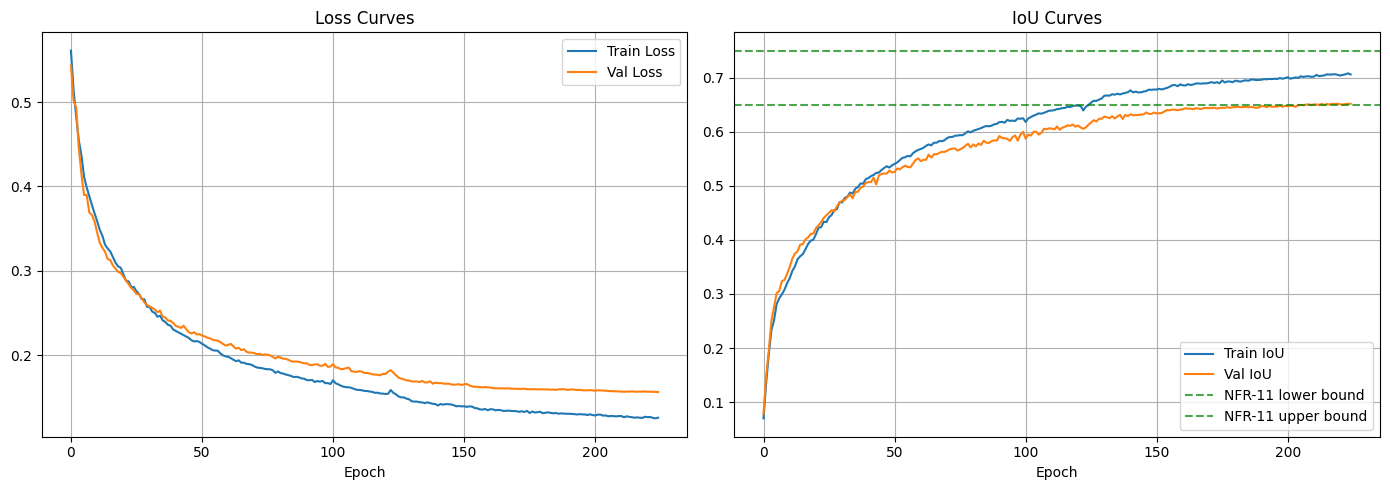
\includegraphics[width=0.98\textwidth]{figures/training_curves.png}
\caption{Training loss and IoU curves for the extended DeepLabV3+ experiment. The dashed green lines represent the NFR-11 target band. Validation IoU enters the target region late in training, while the training curve continues to rise, indicating mild overfitting.}
\label{fig:trainingcurves}
\end{figure*}

Run 4 used a larger SE-ResNeXt-101 encoder and 1024-pixel tiles. The larger receptive field improved performance over baseline but widened the generalization gap, suggesting overfitting due to the smaller number of high-resolution training tiles.

Runs 5 and 6 investigated DeepLabV3+. ASPP improved multi-scale context and AMP reduced memory usage. After extended training, DeepLabV3+ reached 63.05\% test IoU, slightly below the NFR-11 threshold. This suggests the architecture generalizes well but still suffers when trained directly on one-pixel road labels without dilation.

\section{Road Condition Classification}
\subsection{Stage 3b Pipeline Overview}
Manual per-pixel condition annotation is not practical at regional scale. Roadlytics therefore uses an unsupervised-to-supervised strategy. K-Means first generates pseudo-ground-truth condition labels from spectral features. EfficientNet-B2 is then trained to predict those labels from image patches, enabling inference on new imagery.

\subsection{K-Means Pseudo-Labelling}
For each road pixel, six features are extracted: Blue, Green, Red, NIR, NDVI, and mean brightness. NDVI is computed as:
\begin{equation}
\text{NDVI} = \frac{\text{NIR} - R}{\text{NIR} + R}.
\end{equation}
Mean brightness is computed as:
\begin{equation}
\text{Brightness} = \frac{B + G + R}{3}.
\end{equation}
Features are standardized with \texttt{StandardScaler} before clustering. K-Means with $k=3$ produces spectrally coherent clusters that are mapped to Good, Unpaved, and Damaged road semantics through their centroid characteristics.

\subsection{EfficientNet-B2 Classifier}
EfficientNet-B2 was selected for its accuracy-to-parameter efficiency. The first convolutional layer was modified for four-channel input by initializing the NIR channel from the average of pretrained RGB filters. Training patches of $32\times32$ pixels were extracted around road pixels with a 16-pixel stride, producing 102,067 patches. A \texttt{WeightedRandomSampler} balanced mini-batches across classes.

\begin{table}[!t]
\caption{EfficientNet-B2 training configuration.}
\centering
\begin{tabular}{ll}
\toprule
\textbf{Parameter} & \textbf{Value} \\
\midrule
Batch size & 256 \\
Optimizer & AdamW, lr $10^{-3}$, wd $10^{-4}$ \\
LR schedule & CosineAnnealingLR \\
Maximum epochs & 50 \\
Early stopping & 10-epoch patience \\
Loss & CrossEntropyLoss \\
Augmentation & Flips, Rot90, Brightness $\pm10\%$ \\
Best validation accuracy & 82.68\% at epoch 26 \\
\bottomrule
\end{tabular}
\end{table}

\subsection{Test Set Performance}
On 20,414 held-out patches from the training scene, EfficientNet-B2 achieved 83\% accuracy and a macro F1-score of 0.83. The Damaged class had strong overall recall but also showed leakage into Good, reflecting spectral ambiguity between weathered asphalt and intact pavement at 10 m resolution.

\begin{figure}[!t]
\centering
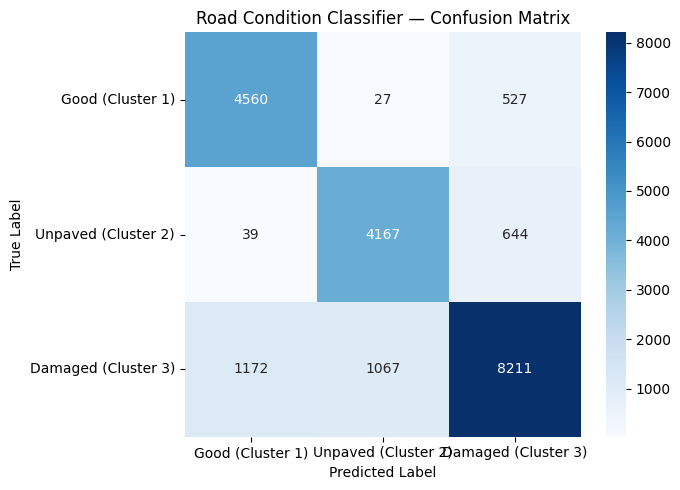
\includegraphics[width=\columnwidth]{figures/condition_confusion_matrix.png}
\caption{EfficientNet-B2 road-condition confusion matrix on held-out test patches. The strong diagonal confirms consistent classification across Good, Unpaved, and Damaged classes, while off-diagonal leakage reflects expected spectral ambiguity at Sentinel-2 resolution.}
\label{fig:conditionconfusion}
\end{figure}

\begin{table}[!t]
\caption{Per-class metrics on held-out EfficientNet-B2 test patches.}
\centering
\begin{tabular}{lcccc}
\toprule
\textbf{Class} & \textbf{Precision} & \textbf{Recall} & \textbf{F1} & \textbf{Support} \\
\midrule
Good & 0.79 & 0.89 & 0.84 & 5,114 \\
Unpaved & 0.79 & 0.86 & 0.82 & 4,850 \\
Damaged & 0.88 & 0.79 & 0.83 & 10,450 \\
Macro avg. & 0.82 & 0.85 & 0.83 & 20,414 \\
Weighted avg. & 0.83 & 0.83 & 0.83 & 20,414 \\
\bottomrule
\end{tabular}
\end{table}

The trained model was also applied to a second unseen Sentinel-2 scene. Predictions were compared against independently generated K-Means pseudo-labels for that scene. Pixel-level agreement reached 72\%, indicating reasonable transferability, although the Unpaved class remained difficult due to inter-scene spectral variation and K-Means label permutation.

\begin{figure}[!t]
\centering
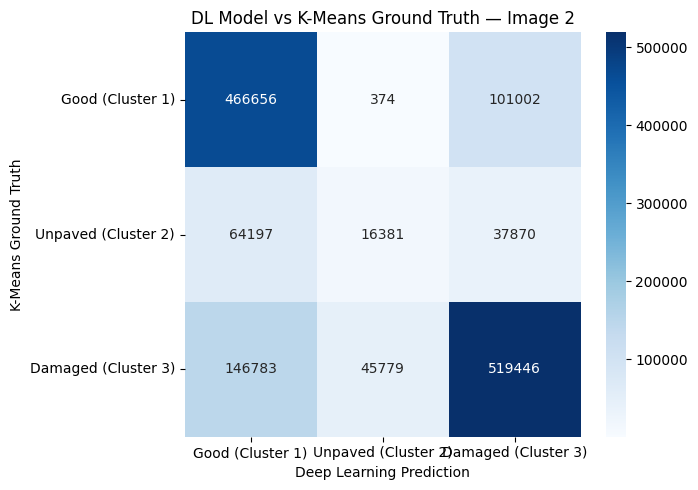
\includegraphics[width=\columnwidth]{figures/unseen_scene_confusion.png}
\caption{Deep-learning predictions compared with independently generated K-Means pseudo-labels on an unseen Sentinel-2 scene. Good and Damaged roads show stronger agreement than Unpaved roads, which are affected by spectral overlap and cluster-label permutation.}
\label{fig:unseenconfusion}
\end{figure}

\section{Roadlytics Web Application}
\subsection{Motivation for Productization}
The original pipeline was notebook- and script-driven, which was appropriate for experimentation but unsuitable for repeatable field-facing use. Roadlytics was therefore productized into a web application with three top-level layers: the geospatial ML pipeline, the backend orchestration layer, and the frontend analysis interface.

\subsection{Application Workflow}
The user uploads a four-band Sentinel-2 Level-2 GeoTIFF in B2, B3, B4, B8 order. The backend validates the file type, band count, and georeferencing. The user then selects a segmentation method, either DeepLabV3 or PakOSM, and a condition-classification method, either K-Means or EfficientNet. The job is processed asynchronously through the states \texttt{uploaded}, \texttt{validating}, \texttt{segmenting}, \texttt{classifying}, \texttt{connectivity}, \texttt{packaging}, and finally \texttt{completed} or \texttt{failed}.

The segmentation output is saved as a GeoTIFF road mask. The classification stage generates four condition outputs: a green Good road mask, a red Unpaved road mask, a yellow Damaged road mask, and a combined condition GeoTIFF containing all three classes. The frontend displays these outputs over the uploaded Sentinel RGB image and a fixed OpenStreetMap basemap. Sentinel RGB and all generated layers are toggleable; the OSM basemap remains fixed.

\subsection{Backend and Storage Architecture}
The backend is implemented with FastAPI and uses SQLite for job metadata, artifacts, events, and analytics snapshots. Azure Blob storage stores uploads, generated GeoTIFFs, reports, and downloadable artifacts. The VM handles orchestration, temporary work directories, and background worker execution. Docker Compose runs the backend, frontend, and Caddy reverse proxy services on the Azure Ubuntu VM.

\subsection{Frontend Interface}
The frontend is implemented in Next.js and provides five main areas: Dashboard, Projects, Processing, Map Analysis, and Reports. Dashboard summarizes recent jobs and system counts. Projects contains the assessment creation flow. Processing shows live job progress and events. Map Analysis renders the OSM basemap, Sentinel RGB, raster masks, connected components, betweenness criticality, and critical junctions. Reports exposes generated HTML summaries and download links.

\begin{figure*}[!t]
\centering
\fbox{\begin{minipage}{0.94\textwidth}
\centering
\textbf{Roadlytics End-to-End Architecture}\\[4pt]
User Uploads Sentinel-2 GeoTIFF $\rightarrow$ FastAPI Validation $\rightarrow$ Background Worker\\
$\rightarrow$ Segmentation (DeepLabV3 or PakOSM) $\rightarrow$ Condition Classification (K-Means or EfficientNet)\\
$\rightarrow$ Raster-First Connectivity Analytics $\rightarrow$ Artifact Packaging $\rightarrow$ Azure Blob + SQLite Metadata\\
$\rightarrow$ Next.js Dashboard / Processing / Map Analysis / Reports $\rightarrow$ RAG Assistant Explanation Layer
\end{minipage}}
\caption{High-level Roadlytics architecture after productization. The RAG assistant sits above the job database, artifact registry, analytics snapshots, report text, and static method notes to provide grounded explanations.}
\label{fig:architecture}
\end{figure*}

\section{RAG Assistant for Roadlytics}
\subsection{Purpose and Scope}
The RAG assistant was added to help users understand what the Roadlytics pipeline produced, why a job failed, which map layers matter, and how to communicate results in reports. The assistant is not a replacement for the ML models or a source of field-confirmed truth. Its role is to translate existing Roadlytics evidence into concise, grounded explanations.

The assistant supports multiple contexts: current job, project library, map analysis, reports, failure help, comparison, and general Roadlytics knowledge. In the user interface, it appears as a floating drawer on Dashboard, Map Analysis, and Reports. On Dashboard, it can summarize the broader workspace and compare recent jobs. On Map Analysis, it receives visible layer names and viewport bounds so it can discuss what the user is currently inspecting. On Reports, it can draft executive summaries, limitations, technical report bullets, and stakeholder-friendly interpretations.

\subsection{Retrieval Sources}
The assistant retrieves from both static and dynamic evidence sources. Static sources include a layer glossary, method notes, upload validation notes, and guardrail notes. Dynamic sources are pulled from the Roadlytics backend database and artifact registry. These include job metadata, selected segmenter and classifier, job status, stage, progress, error messages, event timelines, artifact manifests, layer names, bounds, analytics summaries, and generated HTML report text when available locally.

\begin{table*}[!t]
\caption{RAG evidence sources and their purpose in Roadlytics.}
\centering
\begin{tabularx}{\textwidth}{lYY}
\toprule
\textbf{Evidence Source} & \textbf{Contents} & \textbf{Assistant Use} \\
\midrule
Static method notes & DeepLabV3, PakOSM, K-Means, EfficientNet, layer definitions & Explains model choices and map layer semantics \\
Validation notes & Expected GeoTIFF format, band count, band order, georeferencing & Diagnoses failed uploads and preprocessing issues \\
Guardrail notes & Safety, cost, legal, and field-validation constraints & Prevents unsupported operational claims \\
Job metadata & Project name, status, stage, progress, selected methods, timestamps & Summarizes job state and processing history \\
Job events & Stage-by-stage timeline messages & Explains where a job is stuck or failed \\
Artifact manifest & GeoTIFFs, reports, shapefiles, tile layers, bounds & Connects downloadable outputs to user-facing layers \\
Analytics snapshots & Component counts, critical junction counts, summary metrics & Produces report summaries and prioritization guidance \\
Report text & Generated HTML report converted to plain text & Drafts narrative summaries and stakeholder explanations \\
Map context & Visible layers and viewport bounds & Answers map-specific questions using current UI state \\
\bottomrule
\end{tabularx}
\end{table*}

\subsection{Indexing and Retrieval Design}
Each evidence item is converted into an \texttt{EvidenceChunk} containing a source, label, text body, and metadata. Long text, such as generated report content, is split into chunks of approximately 1,300 characters. Chunks are inserted into a persistent ChromaDB collection named \texttt{roadlytics\_assistant}. The Chroma persistence path is configured through \texttt{ROADLYTICS\_ASSISTANT\_CHROMA\_PATH} and defaults to \texttt{/app/backend/data/chroma} inside Docker, which is mounted to persistent backend storage.

A practical deployment constraint was avoiding additional model downloads on the Azure VM. Instead of relying on Chroma's default embedding model, Roadlytics uses a deterministic local hash embedding function. Tokens are hashed into a fixed 256-dimensional vector with signed accumulation and normalization. This gives semantic-ish lexical retrieval behavior without requiring a GPU, external embedding API, or local embedding model download. If Chroma is unavailable or retrieval fails, the assistant falls back to lexical overlap scoring over the same evidence chunks.

\subsection{Generation Layer}
When \texttt{GEMINI\_API\_KEY} is configured, the backend uses the \texttt{google-genai} Python package to call the configured Gemini model. The default model is \texttt{gemini-2.5-flash}, selected because it is fast and suitable for free-tier-friendly interactive summaries. The prompt includes the assistant mode, job identifiers, comparison job identifier, visible map layers, viewport bounds, and the retrieved evidence capped by \texttt{ROADLYTICS\_ASSISTANT\_MAX\_CONTEXT\_CHARS}. The default context cap is 18,000 characters.

If the Gemini key is missing, the package is unavailable, or the provider returns an error, the assistant returns an extractive fallback answer from the retrieved Roadlytics evidence. This design prevents the UI from failing completely during local development, expired-key scenarios, or constrained deployments. The response records the provider as either \texttt{gemini} or \texttt{local-fallback}, and the model as either the configured Gemini model or \texttt{extractive}.

\subsection{API and Frontend Integration}
The backend exposes three assistant endpoints:
\begin{itemize}
\item \texttt{POST /api/assistant/chat}: accepts a user message, mode, job identifier, optional comparison job identifier, visible layer names, viewport bounds, and conversation identifier.
\item \texttt{GET /api/assistant/suggestions}: returns mode-specific starter prompts.
\item \texttt{POST /api/assistant/reindex}: rebuilds the assistant index over available Roadlytics evidence.
\end{itemize}

The frontend uses a reusable \texttt{AssistantDrawer} component. It stores chat state on the client, sends structured requests to the backend, displays assistant answers, shows retrieved evidence citations, and exposes mode-specific quick prompts. For example, Map Analysis suggests questions such as ``Summarize the visible layers'' and ``What should be inspected first?'' Reports suggests ``Write an executive summary'' and ``List the key limitations.''

\subsection{Guardrails and Decision-Support Boundaries}
The assistant prompt explicitly instructs the model to answer only from Roadlytics evidence and method notes. It must not invent exact repair costs, legal compliance conclusions, guaranteed road safety, emergency routing reliability, or field-confirmed truth. The backend appends a required caveat to analytical responses: outputs are based on uploaded imagery and Roadlytics model predictions, and field inspection is required before operational decisions.

This guardrail design is important because Roadlytics operates on 10 m remote-sensing imagery and model-derived masks. The assistant can explain what the models produced and what artifacts indicate, but it cannot certify pavement condition, assign legal responsibility, or replace civil-engineering inspection.

\subsection{RAG Workflow}
\begin{figure*}[!t]
\centering
\fbox{\begin{minipage}{0.94\textwidth}
\centering
\textbf{Roadlytics RAG Flow}\\[4pt]
User Question + UI Context $\rightarrow$ Assistant Request Schema $\rightarrow$ Evidence Builder\\
$\rightarrow$ Static Docs + SQLite Job Data + Artifacts + Analytics + Report Text\\
$\rightarrow$ Chunking $\rightarrow$ ChromaDB Hash-Embedding Retrieval $\rightarrow$ Prompt Assembly\\
$\rightarrow$ Gemini Generation or Local Extractive Fallback $\rightarrow$ Answer + Citations + Caveats + Recommended Actions
\end{minipage}}
\caption{The Roadlytics assistant is retrieval-first. Generation is constrained by retrieved evidence and backed by explicit citations and limitations.}
\label{fig:ragflow}
\end{figure*}

\subsection{Assistant Capabilities}
The implemented assistant supports the following practical workflows:
\begin{itemize}
\item \textbf{Assessment summarization}: converts job metadata, analytics, and report text into concise explanations.
\item \textbf{Map-layer interpretation}: explains Sentinel RGB, segmentation masks, condition masks, connected components, betweenness criticality, and critical junctions.
\item \textbf{Failure diagnosis}: uses job errors and event timelines to explain upload validation failures or processing-stage failures.
\item \textbf{Report drafting}: produces executive summaries, limitation statements, and technical bullets from completed job evidence.
\item \textbf{Project-library reasoning}: summarizes recent jobs and identifies which completed assessment may require closer inspection based on available metadata.
\item \textbf{Comparison mode}: accepts a primary and comparison job identifier for side-by-side explanation when both are provided.
\item \textbf{Guarded recommendations}: suggests actions such as reviewing combined condition masks, inspecting damaged layers, and prioritizing critical junctions while preserving field-validation caveats.
\end{itemize}

\subsection{Deployment Configuration}
The assistant is configured through Docker environment variables. The key variables are \texttt{GEMINI\_API\_KEY}, \texttt{ROADLYTICS\_ASSISTANT\_MODEL}, \texttt{ROADLYTICS\_ASSISTANT\_EMBEDDING\_MODEL}, \texttt{ROADLYTICS\_ASSISTANT\_CHROMA\_PATH}, and \texttt{ROADLYTICS\_ASSISTANT\_MAX\_CONTEXT\_CHARS}. The Azure VM deployment requires adding the Gemini API key to \texttt{/opt/roadlytics/deploy/azure/.env.vm} and rebuilding the backend image because the assistant introduces the \texttt{google-genai} and \texttt{chromadb} Python dependencies.

\section{Discussion}
\subsection{Architecture vs. Data Representation}
The most important modelling finding is that data representation outweighed architectural complexity. A simple $3\times3$ label dilation produced a larger IoU gain than switching to deeper encoders or more complex segmentation heads. This result is significant because it demonstrates that the dominant bottleneck was not raw model capacity, but the geometric degeneracy of one-pixel road labels at Sentinel-2 resolution.

\subsection{Unpaved Class Transferability}
The Unpaved class underperformed on the unseen scene. Two explanations are likely. First, K-Means labels can be permuted between scenes because clustering is performed independently. Second, unpaved roads in Sindh have high intra-class spectral variance, ranging from bright compacted sand to darker muddy tracks. A future centroid-transfer strategy would reduce label permutation and improve cross-scene consistency.

\subsection{Tree Shadow Misclassification}
Tree-lined roads are vulnerable to misclassification because canopy shadows reduce NIR reflectance and alter NDVI. K-Means can therefore assign shaded asphalt to the Damaged class even when pavement is intact. Multi-temporal compositing, explicit shadow detection, or Sentinel-1 SAR fusion could mitigate this limitation.

\subsection{RAG Reliability and Limits}
The RAG assistant improves usability but does not improve the underlying model outputs. Its reliability depends on the quality of the indexed evidence and the correctness of job metadata, artifact registration, and analytics snapshots. The local hash embedding strategy is intentionally lightweight and deployment-friendly, but it is less semantically expressive than a dedicated embedding model. This trade-off is acceptable for phase one because Roadlytics evidence is structured, domain-specific, and relatively compact. If the document base grows substantially, a stronger embedding model or managed vector database could improve retrieval quality.

\section{Conclusions and Future Work}
\subsection{Summary of Achievements}
Roadlytics satisfies NFR-11 with a 66.2\% test IoU segmentation result using U-Net/ResNet-34 and training-time label dilation. The road-condition classifier achieves 83\% test accuracy and macro F1 of 0.83 across Good, Unpaved, and Damaged classes. The project further productizes the research pipeline into a deployable web application with FastAPI, Next.js, Docker, Azure VM hosting, Azure Blob storage, OSM basemap visualization, GeoTIFF artifacts, report generation, and a grounded RAG assistant.

\subsection{Future Work}
High-priority modelling work includes applying label dilation to DeepLabV3+, adding test-time augmentation, introducing Sentinel-1 SAR fusion, and implementing cross-scene K-Means centroid transfer. High-priority product work includes persistent user accounts, managed job queues, richer report exports, stronger retrieval embeddings, and assistant conversation memory. A future topology-refinement model, such as a diffusion or conditional GAN post-processor, could bridge short segmentation gaps and enforce graph-theoretic plausibility before condition classification.

\section*{Reproducibility}
All model experiments used fixed random seed 42 for NumPy, PyTorch, and Python. Tile generation, model definitions, training loops, and evaluation scripts are documented in the accompanying Roadlytics notebooks and source repository. The deployed application uses Docker Compose for repeatable backend, frontend, and reverse-proxy startup. The assistant can operate with Gemini generation when configured or with local extractive fallback when no API key is present.

\begin{thebibliography}{00}
\bibitem{unet} O. Ronneberger, P. Fischer, and T. Brox, ``U-Net: Convolutional Networks for Biomedical Image Segmentation,'' in \emph{MICCAI}, 2015.
\bibitem{deeplab} L.-C. Chen, Y. Zhu, G. Papandreou, F. Schroff, and H. Adam, ``Encoder-Decoder with Atrous Separable Convolution for Semantic Image Segmentation,'' in \emph{ECCV}, 2018.
\bibitem{efficientnet} M. Tan and Q. Le, ``EfficientNet: Rethinking Model Scaling for Convolutional Neural Networks,'' in \emph{ICML}, 2019.
\bibitem{focal} T.-Y. Lin, P. Goyal, R. Girshick, K. He, and P. Dollar, ``Focal Loss for Dense Object Detection,'' in \emph{ICCV}, 2017.
\bibitem{dice} F. Milletari, N. Navab, and S.-A. Ahmadi, ``V-Net: Fully Convolutional Neural Networks for Volumetric Medical Image Segmentation,'' in \emph{3DV}, 2016.
\bibitem{rag} P. Lewis et al., ``Retrieval-Augmented Generation for Knowledge-Intensive NLP Tasks,'' in \emph{NeurIPS}, 2020.
\bibitem{repaint} A. Lugmayr et al., ``RePaint: Inpainting using Denoising Diffusion Probabilistic Models,'' in \emph{CVPR}, 2022.
\bibitem{pix2pix} P. Isola, J.-Y. Zhu, T. Zhou, and A. A. Efros, ``Image-to-Image Translation with Conditional Adversarial Networks,'' in \emph{CVPR}, 2017.
\end{thebibliography}

\end{document}

